The Image processing app splits into two parts. An external server which provides the infrastructure to store and distribute bitstreams and 
the android app (client) which interacts with the server and the hardware on the zedboard. 

\subsubsection{Client aplication}

The client is a native android application written in Android Studio version 3.2.1 for Android API 10 (Gingerbread 2.3.3).
Unfortunately todays Android SDK (API 28) does not support Gingerbread anymore, version 25 was the last SDK that officially supports Gingerbread. To compile for Gingerbread set compileSdkVersion to 25 with the
targetSdk set to 10 as seen in~\Cref{lst:appbuild}.
\begin{lstlisting}[
	language=Bash,
	caption={App build setup},
	label={lst:appbuild},
	basicstyle=\small
	]
apply plugin: 'com.android.application'
android {
    compileSdkVersion 25
    defaultConfig {
        applicationId "com.lab.soc.client"
        minSdkVersion 10
        targetSdkVersion 10
        versionCode 1
        versionName "1.0"
        testInstrumentationRunner "android.support.test.runner.AndroidJUnitRunner"
    }
    buildTypes {
        release {
            minifyEnabled false
            proguardFiles getDefaultProguardFile('proguard-android.txt'), 
            'proguard-rules.pro'
        }
    }
    buildToolsVersion '28.0.3'
}

dependencies {
    implementation fileTree(include: ['*.jar'], dir: 'libs')
    implementation 'com.android.support:appcompat-v7:25.4.0'
    implementation 'com.android.support.constraint:constraint-layout:1.1.3'
    implementation 'com.android.support:support-v4:25.4.0'
    testImplementation 'junit:junit:4.12'
    androidTestImplementation 'com.android.support.test:runner:1.0.2'
    androidTestImplementation 'com.android.support.test.espresso:espresso-core:3.0.2'
}    
\end{lstlisting}
This way it is possible to use Google's support libraries, which deliver
backward compatibility for newer Android classes (e.g fragments) and allows to run the app on all Android versions from Gingerbread to Pie without version specific modifications. Whenever possible Androids own APIs has been used, if not available on Gingerbread they were replaced with own implementations.\newline

The architecture is following the single responsibility principle, separating the concerns into several classes:

\begin{itemize}
    \item MainActivity 	    - Android specific (UI,Events,Life cycle,)
    \item NetworkManager	- Network operations 
    \item MsgProcessor	    - JSON processing 
    \item FabricManager	    - PL Fabric interaction
    \item AppExecutors	    - Multi threading
    \item Util			    - Utility (Image preprocessing)
    \item Repository        - Data format
\end{itemize}


The Network Manager spawns a new thread and opens a connection to the server. Then requests new information using the REST API (see server section). The received information is packed inside a JSON object (JavaScript Object Notation) and forwarded to the MsgProcessor. Where they are unpacked,compared and saved.

Example JSON object:
\begin{verbatim}
{
    "Index": "SOC-LAB-IOT",
    "Title": "IOT Image Processing",
    "Version": "002",
    "Description": "",
    "Changelog": ["3.11.2018 Primary release", 
                    "4.11.2018 Bug fixing", 
                    "6.11.2018 added stuff"],
    "File": "filter_0_0_4.bin",
    "Date": "6.11.2018",
    "Checksum": "fdg851dfg654dfg6541dfg65514dfghdfg45534terg"
}  
\end{verbatim}



If there is a new version available, the Network Manager will download the new bitstream from the sever using the REST API (see server section). The Fabric Manager will then calculate the hash from the bitstream file on the programmable logic. If they match, the PL fabric will be reconfigured with the downloaded bitstream. In a real world scenario, the whole process would run in the background without user interference. For demonstration purposes a simple user interface was implemented to trigger the download and apply filters on a test picture.

\begin{figure}[h]
\centering
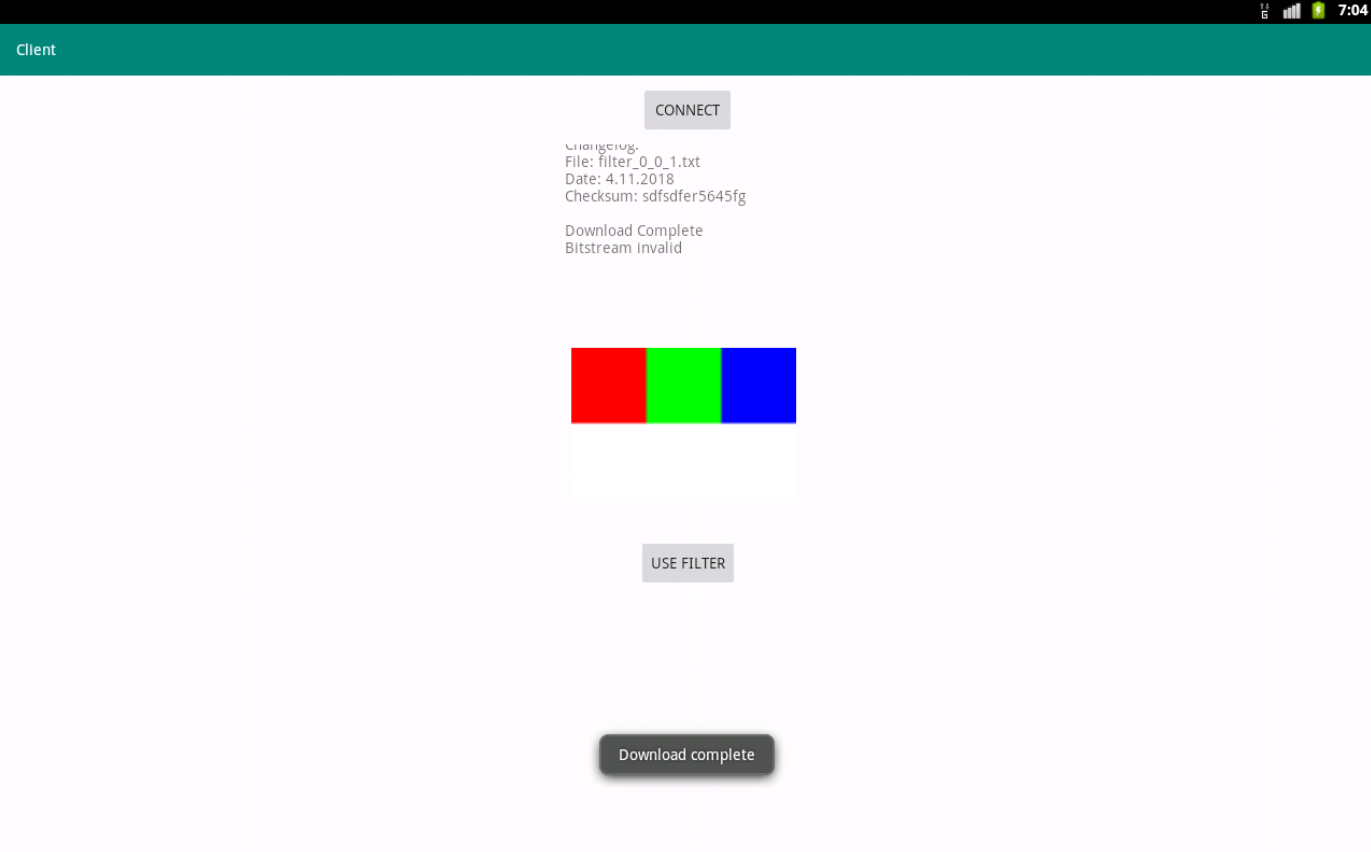
\includegraphics[width=1\textwidth]{sections/methodology/clientdownload.png}
\caption{\label{fig:gic} user interface}
\end{figure}

To apply filters the app has to pre process the image for the device driver to the following specification:
32 bit integer
ALPHA | RED |GREEN | BLUE (8bit|8bit|8bit|8bit) e.g full opaque red would be (hex notation) FF FF 00 00. Every pixel will be read out and saved together to a new binary file. 
The path to this file will be written to the device driver, soon after the filtered data will be read back into the UI from the same file.


\subsubsection{Server}

A tiny webserver with a REST API (Representational State Transfer), 
written with python 3.7 using Flask and its extension FlaskRESTful, therefore fully WSGI compliant
(Webserver Gateway Interface). However Flask internal development server is used for the demonstration and for simplicity.

To start the server, open a terminal in the server directory. Type in following command:
\begin{verbatim}
Flask run -h *your ip* -p 5000    
\end{verbatim}
Open http://*your ip*:5000 to see if the server is reachable

\subsubsection{Server API}

Insomnia, a free open source REST client available for Mac,Windows and Linux, was used for API testing and server communication.

\begin{figure}[h]
\centering
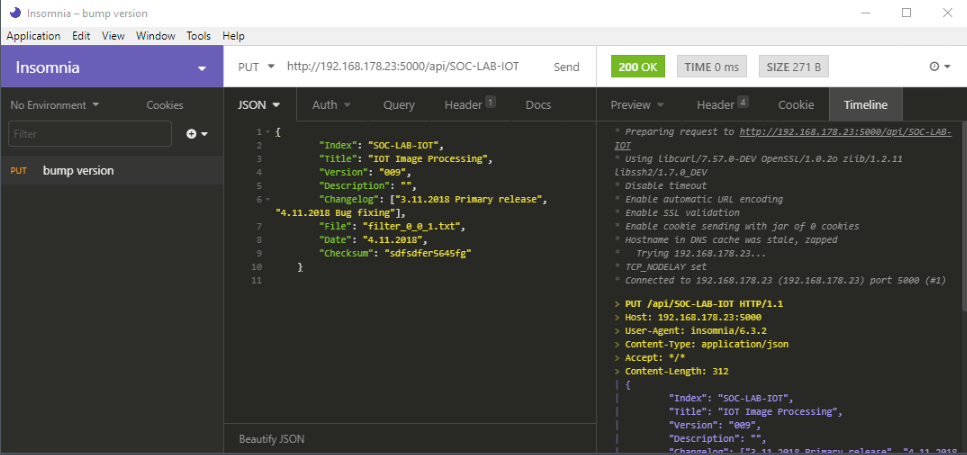
\includegraphics[width=1\textwidth]{sections/methodology/insomnia.png}
\caption{\label{fig:gic2} Insomnia}
\end{figure}



\newcommand{\specialcell}[2][c]{%
  \begin{tabular}[#1]{@{}c@{}}#2\end{tabular}}
  
\subsubsubsection{Get all information for repository <index>:}
\begin{table}[h]
    \begin{tabular}[h]{llllll}
    URL          & \specialcell{URL\\PARAM}     & \specialcell{DATA\\PARAM}  & METHOD &  \specialcell{SUCCESS\\RESPONSE} & \specialcell{ERROR\\RESPONSE} \\ \hline
    /api/<index> & index=[string] & n/a    & GET   & 200              & 404            \\ 
    \end{tabular}
\end{table}



\subsubsubsection{Create repository <index>:}
\begin{table}[h]
    \begin{tabular}[h]{llllll}
    URL          & \specialcell{URL\\PARAM}     & \specialcell{DATA\\PARAM}  & METHOD &  \specialcell{SUCCESS\\RESPONSE} & \specialcell{ERROR\\RESPONSE} \\ \hline
    /api/<index> & index=[string] & JSON    & POST   & 201              & 400            \\ 
    \end{tabular}
\end{table}

JSON:
\begin{verbatim}
{
    "Index": "SOC-LAB-IOT",
    "Title": "IOT Image Processing",
    "Version": "001",
    "Description": "",
    "Changelog": ["3.11.2018 Primary release", "4.11.2018 Bug fixing"],
    "File": "filter_0_0_1.txt",
    "Date": "4.11.2018",
    "Checksum": ""
}	    
\end{verbatim}

\subsubsubsection{Update repository <index> or create it if not existing:}
\begin{table}[h]
    \begin{tabular}[h]{llllll}
    URL          & \specialcell{URL\\PARAM}     & \specialcell{DATA\\PARAM}  & METHOD &  \specialcell{SUCCESS\\RESPONSE} & \specialcell{ERROR\\RESPONSE} \\ \hline
    /api/<index> & index=[string] & JSON  & PUT    & 200              & 201            \\ 
    \end{tabular}
\end{table}

JSON:
\begin{verbatim}
{
    "Index": "SOC-LAB-IOT",
    "Title": "IOT Image Processing",
    "Version": "002",
    "Description": "",
    "Changelog": ["3.11.2018 Primary release", 
    "4.11.2018 Bug fixing", 
    "6.11.2018 added stuff"],
    "File": "filter_0_0_4.bin",
    "Date": "6.11.2018",
    "Checksum": "fdg851dfg654dfg6541dfg65514dfghdfg45534terg"
}	
\end{verbatim}

\subsubsubsection{Delete repository <index>:}

\begin{table}[h]
    \begin{tabular}[h]{llllll}
    URL          & \specialcell{URL\\PARAM}     & \specialcell{DATA\\PARAM}  & METHOD &  \specialcell{SUCCESS\\RESPONSE} & \specialcell{ERROR\\RESPONSE} \\ \hline
    /api/<index> & index=[string] & n/a        & DELETE & 200              & 404            \\ 
    \end{tabular}
\end{table}

\subsubsubsection{Download file <filename>}
\begin{table}[h]
    \begin{tabular}[h]{llllll}
    URL          & \specialcell{URL\\PARAM}     & \specialcell{DATA\\PARAM}  & METHOD &  \specialcell{SUCCESS\\RESPONSE} & \specialcell{ERROR\\RESPONSE} \\ \hline
    \specialcell{/api/download/\\<path:filename>} &  filename=[string] & n/a        & GET    & 200              & 404            \\ 
    \end{tabular}
\end{table}
